\begin{frame}{Linear Systems and Direct Methods}
  

  \vspace{-0.2cm}

  \begin{center}

    \begin{block}{Sparse linear systems}
      Many applications from physics, engineering, chemistry, geodesy,
      etc, require the solution of a linear system like

      \vspace{0.2cm}

      % $Ax = b,~~A\in \mathbb{R}^{m\times m}$ or
      $Ax = b$

      \vspace{0.1cm}

      % $\min_x \|Ax-b\|_2,~~A\in \mathbb{R}^{m\times n},~~m>n$
      $\min_x \|Ax-b\|_2$

      % \begin{flalign*}
        % & Ax = b,~~A\in \mathbb{R}^{m\times m} \\
        % & \min_x \|Ax-b\|_2,~~A\in \mathbb{R}^{m\times n},~~m>n
      % \end{flalign*}

      \vspace{0.2cm}

      where A is \dr{large} and \dr{sparse}.
    \end{block}
    
    \vspace{0.3cm}

    \begin{columns}
      \begin{column}{0.05\textwidth}
      \end{column}
      \begin{column}{0.7\textwidth}
        
        % \begin{block}{Sparsity}          
          
          A sparse matrix is mostly filled with zeros:
          \begin{itemize}
          \item Reduce \dr{memory} storage.
          \item Reduce \db{computational costs}.
          \item Generate \dg{parallelism}.
          \end{itemize}
          
        % \end{block}
      \end{column}
      \begin{column}{0.25\textwidth}
          
        \includegraphics[width=0.8\textwidth]{figures/Maragal_4.pdf}
        
      \end{column}
    \end{columns}
          

    % \begin{columns}
    %   \begin{column}{0.6\textwidth}
        
    %     \begin{block}{Sparsity}          
    %       A sparse matrix is mostly filled with zeros:
    %       \begin{itemize}
    %       \item Reduce \dr{Memory} storage.
    %       \item Reduce \dr{computational costs}.
    %       \item Generate \dr{parallelism}.
    %       \end{itemize}
          
    %     \end{block}
    %   \end{column}
    %   \begin{column}{0.4\textwidth}
    %     \centering
    %     \begin{figure}
    %       \includegraphics[width=0.5\textwidth]{Maragal_4.pdf}
    %       %\caption{Least squares problem.}
    %     \end{figure}
    %   \end{column}

    % \end{columns}
  \end{center}

\end{frame}

\begin{frame}{Linear Systems solution: methods}

  \begin{block}{Direct methods}
    Based on the factorization of the input matrix:

    \begin{itemize}
    \item[\dg{$\blacktriangle$}] Numerically robust, large set of
      features, general purpose.
    \item[\dr{$\blacktriangledown$}] High memory consumption and
      computational cost.
    \end{itemize}
  \end{block}

  \begin{block}{Iterative methods}
    Iteratively refine an initial guess of the solution:

    \begin{itemize}
    \item[\dg{$\blacktriangle$}] Fast, low memory usage.
    \item[\dr{$\blacktriangledown$}] Not always reliable.
    \end{itemize}
  \end{block}

  \begin{block}{Direct-iterative hybrid methods}
    Combine the advantages of direct and iterative methods:
    \begin{itemize}
    \item[\dg{$\blacktriangle$}] More scalable and less costly than direct methods, 
    \item[\dr{$\blacktriangledown$}]  but less robust and general purpose.
    \end{itemize}
  \end{block}

  % \begin{itemize}
  % \item \dr{Direct methods}: factorization-based method e.g. $A = QR$
    % \begin{itemize}
    % \item[\dg{$\blacktriangle$}] Numerically robust
    % \item[\dr{$\blacktriangledown$}] Memory footprint, computational
      % cost
    % \end{itemize}
  % \item \dr{Iterative methods}:
    % \begin{itemize}
    % \item[\dg{$\blacktriangle$}] Fast, low memory usage
    % \item[\dr{$\blacktriangledown$}] Not always reliable
    % \end{itemize}
  % \item \dr{Direct-iterative hybrid methods}: Fast and scalable by
    % taking advantage of both direct and iterative methods.
  % \end{itemize}

\end{frame}

%% Architectures

\begin{frame}{Architectures}
  \begin{center}
    \only<1>{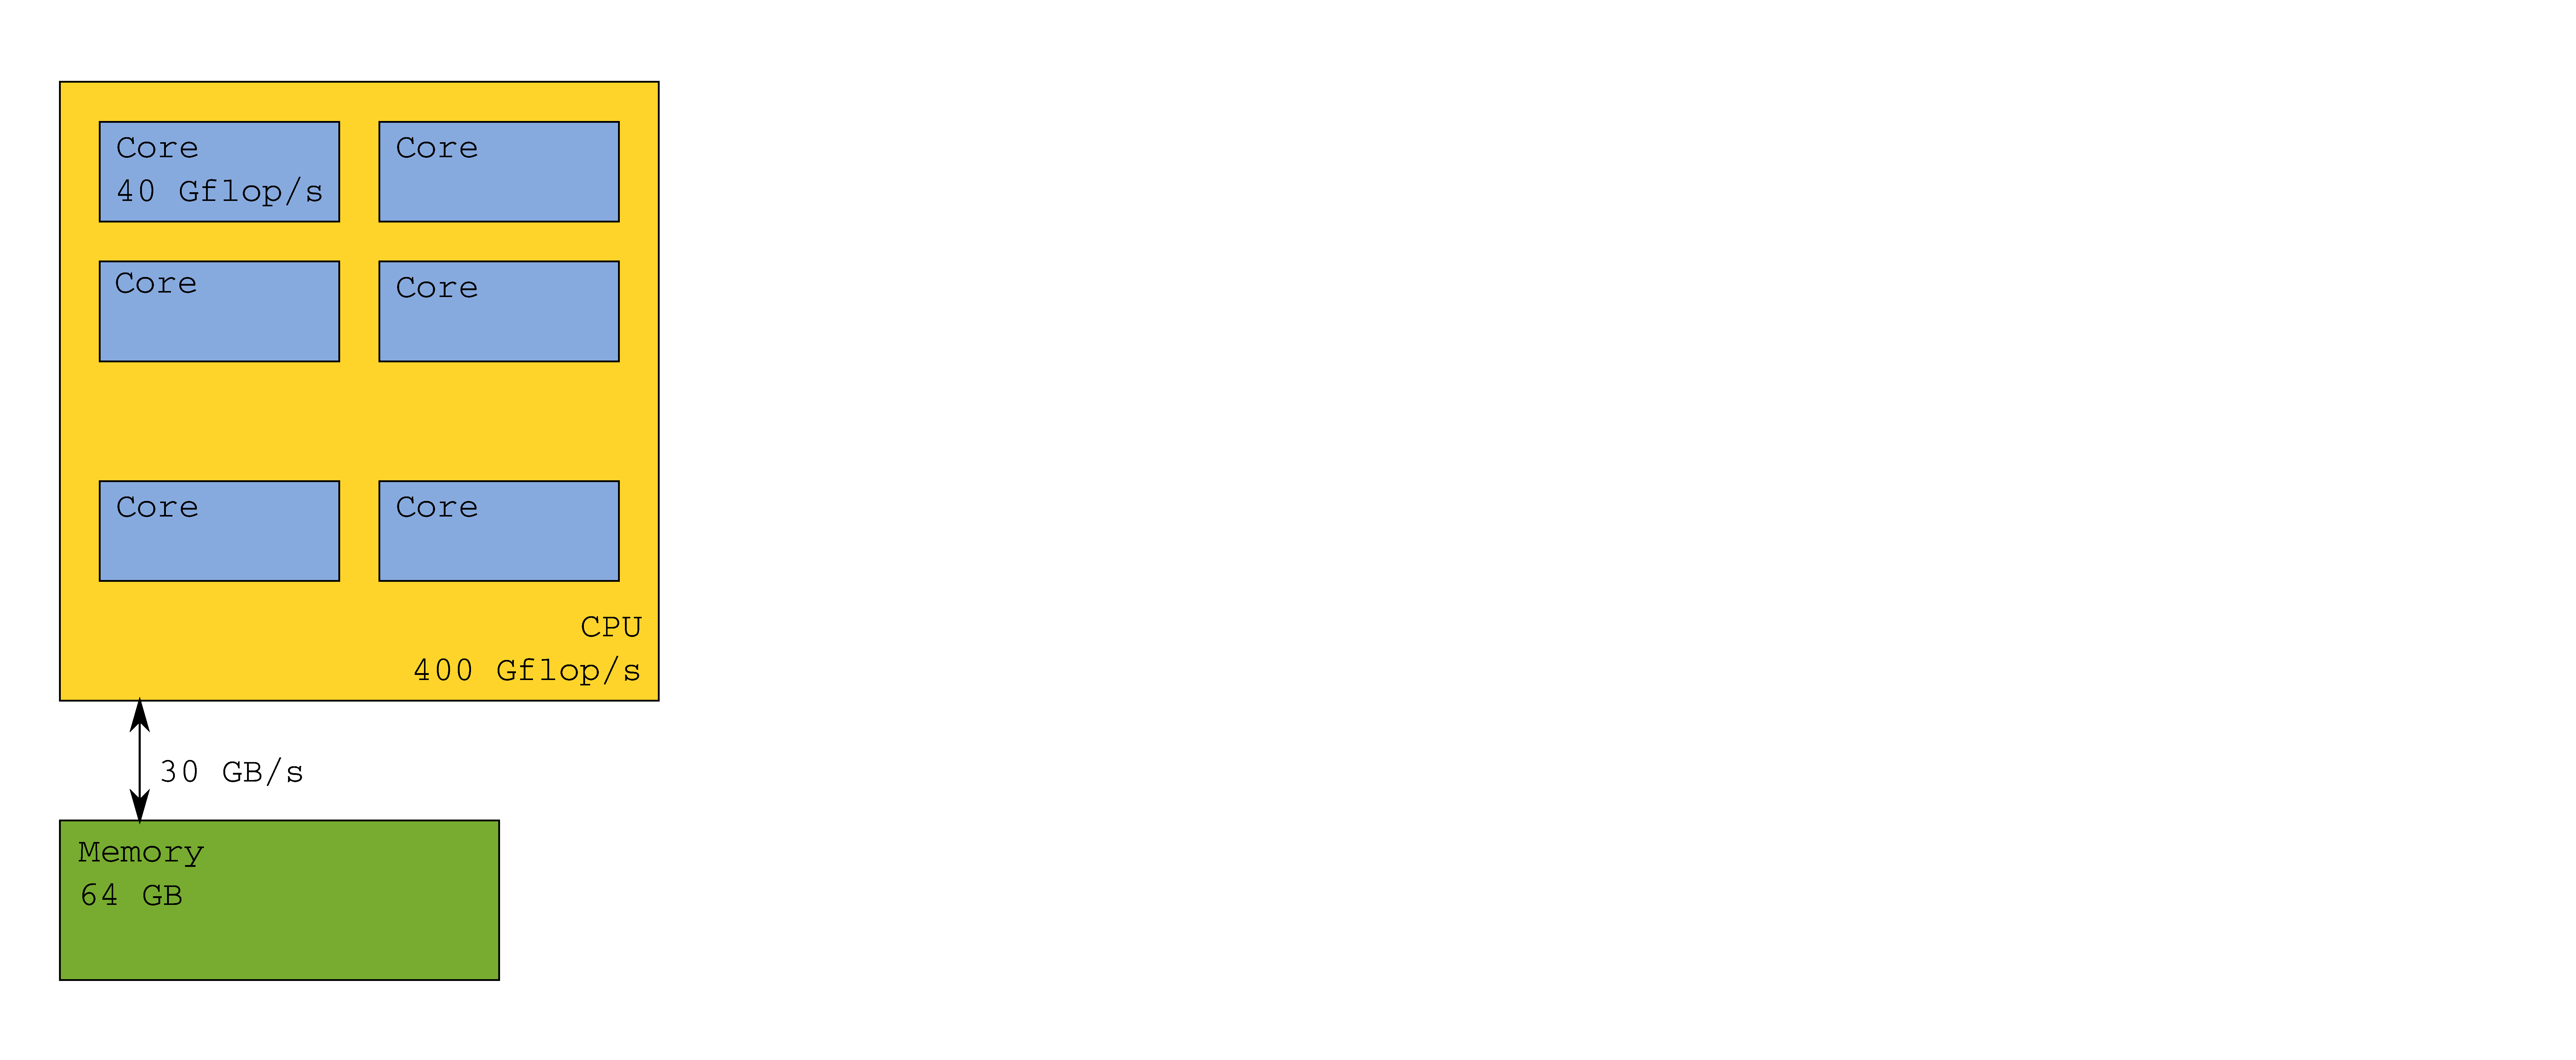
\includegraphics[width=0.9\textwidth]{figures/hpc-arch1}}%
    \only<2>{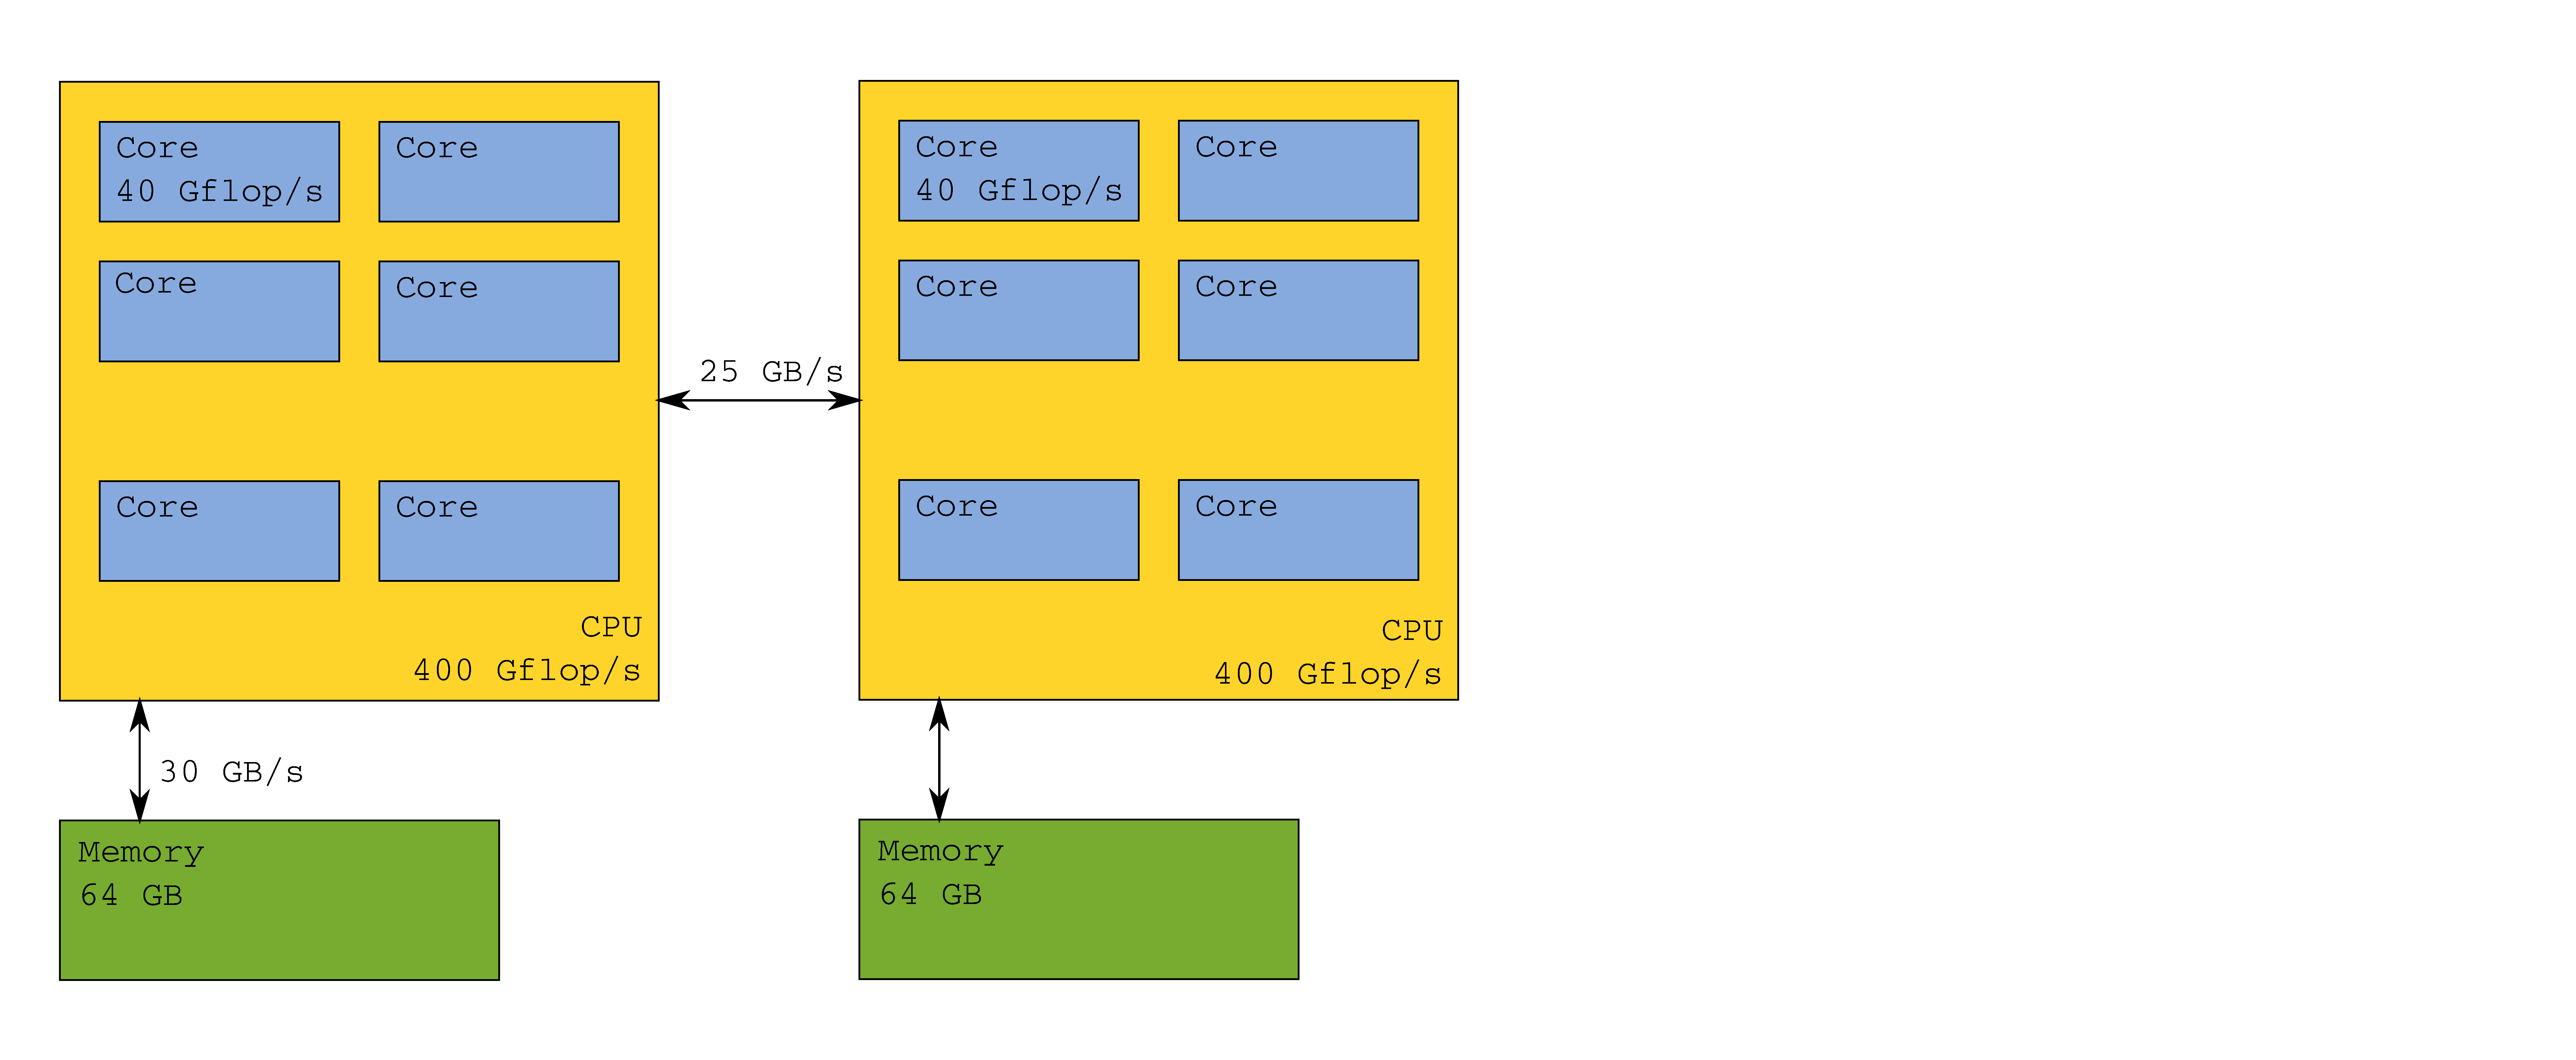
\includegraphics[width=0.9\textwidth]{figures/hpc-arch2}}%
    \only<3>{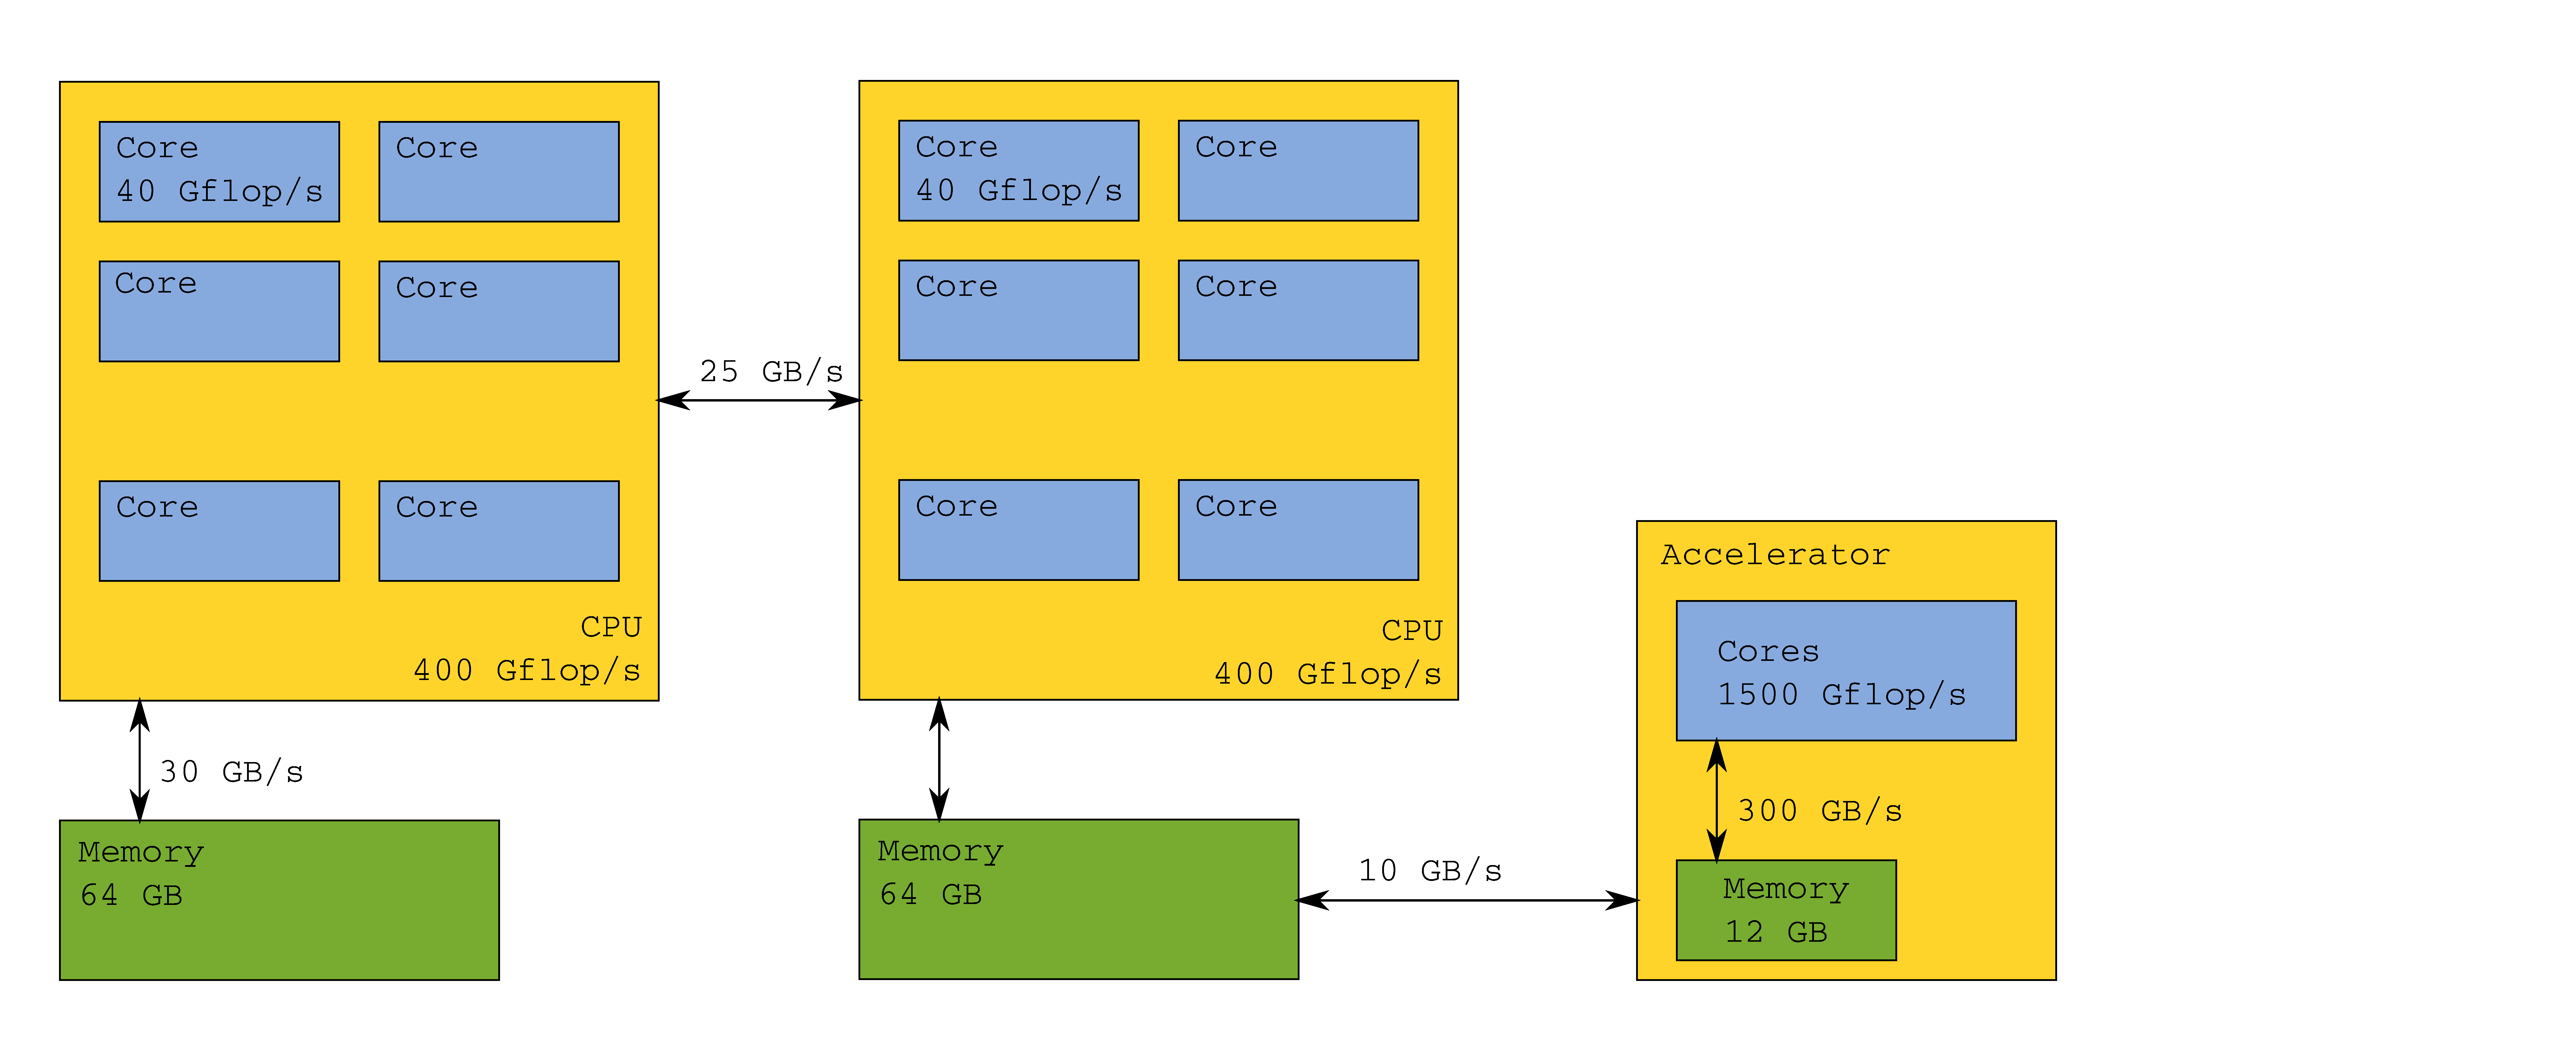
\includegraphics[width=0.9\textwidth]{figures/hpc-arch3}}%
    \only<4->{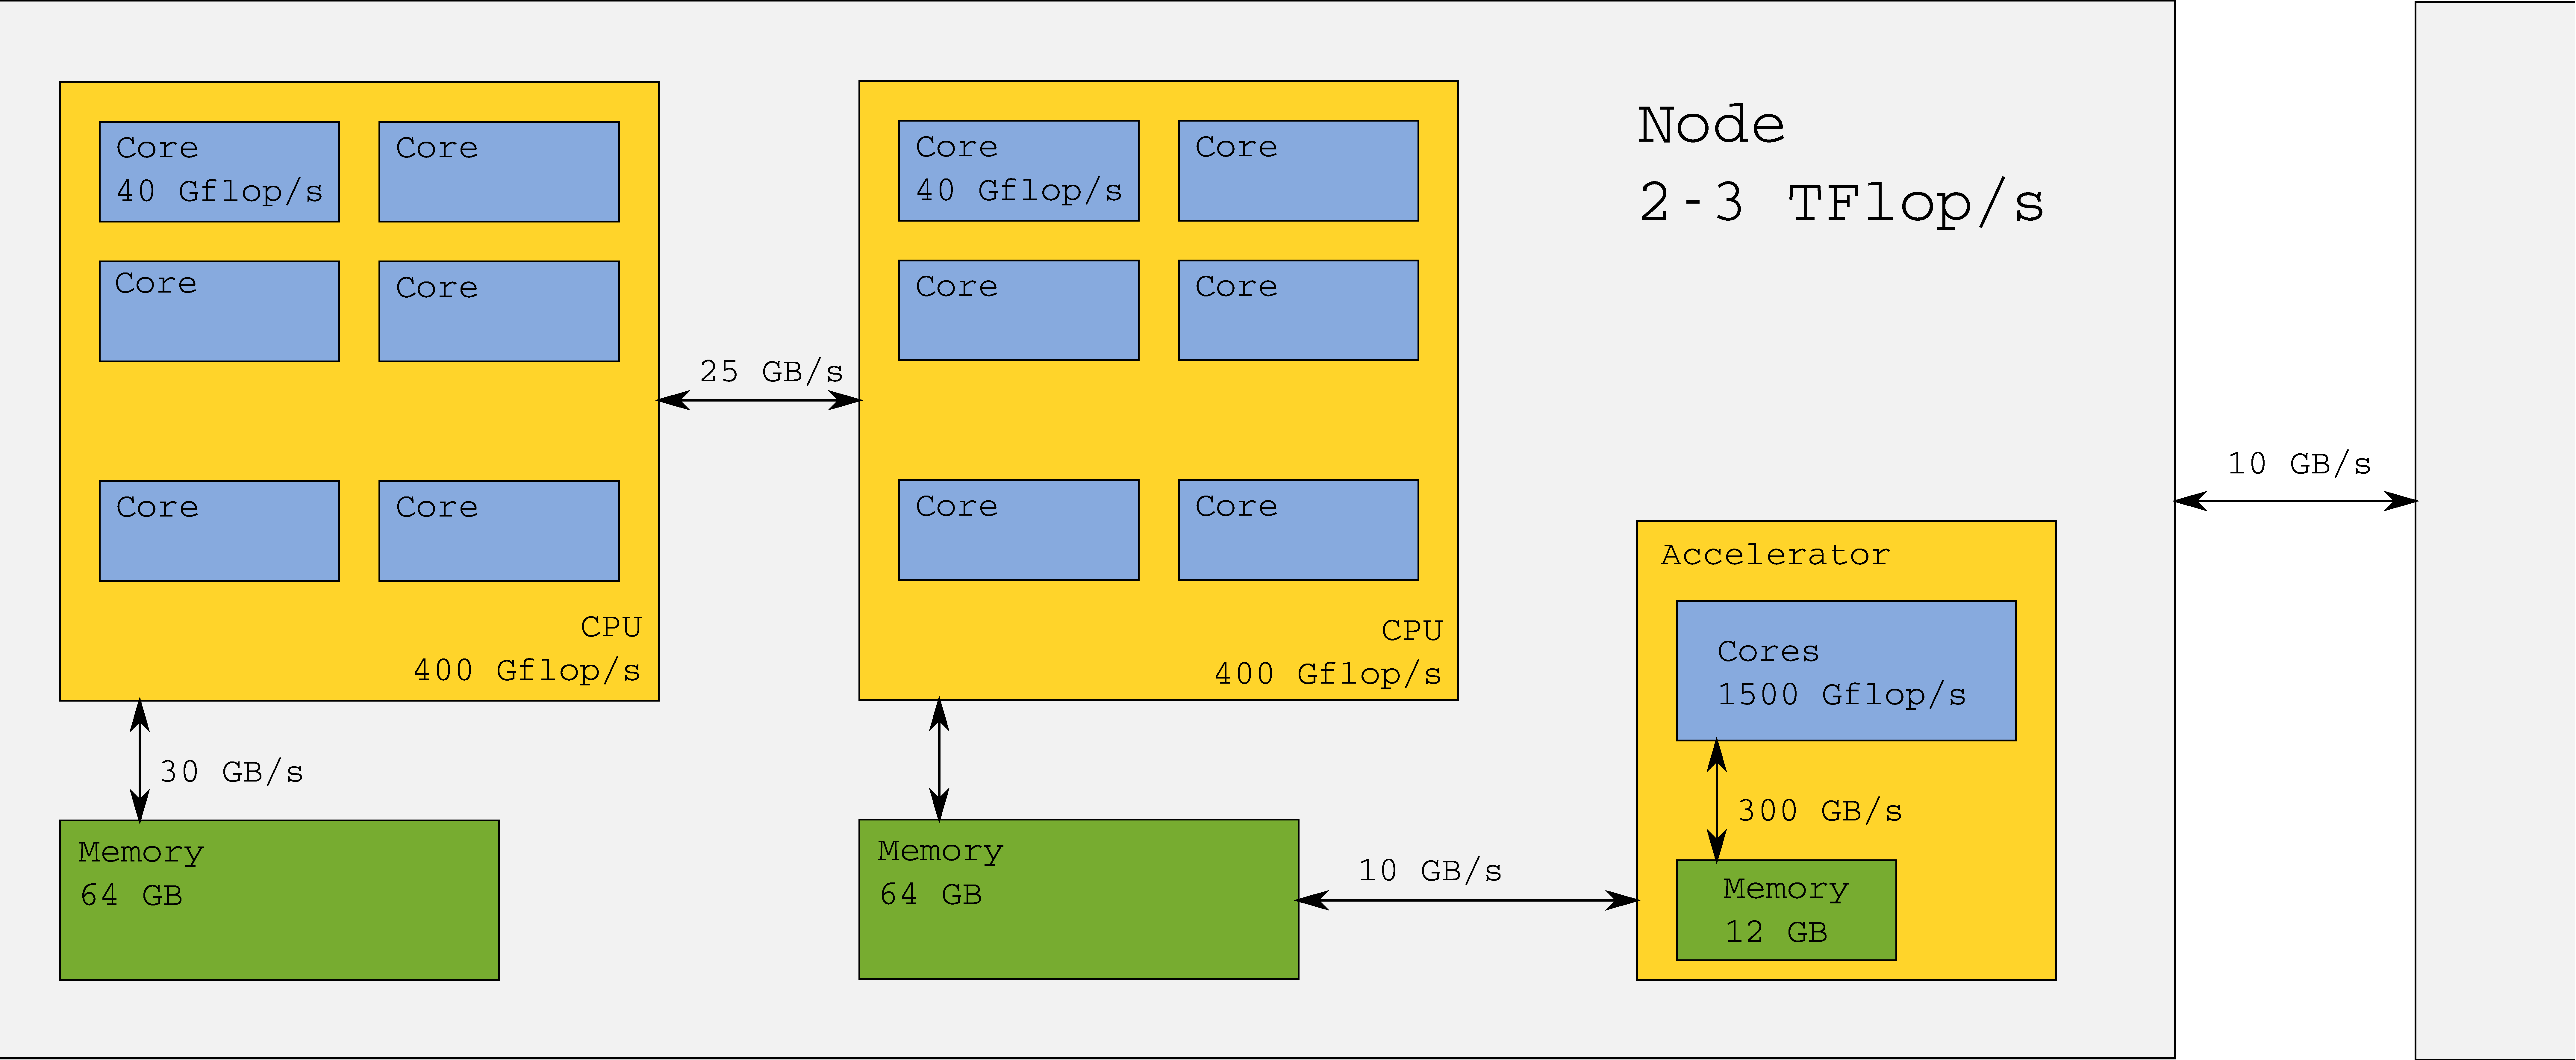
\includegraphics[width=0.9\textwidth]{figures/hpc-arch4}}%
  \end{center}
    
  Typical HPC computing platforms are equipped with
  multiple nodes, connected through a high speed network, with at
  each nodes:
  \begin{itemize}
  \item<1-> \dr{multicore processors} connected to a NUMA memory node.
  \item<3-> one or more \dr{accelerators}.
  \end{itemize}
  \uncover<5>{Current HPC platform are extremely \db{heterogeneous} with
    diverse resource capabilities and memory speeds offered by these
    architectures.}  

\end{frame}

% \begin{frame}{Architectures}

%   \begin{center}
%    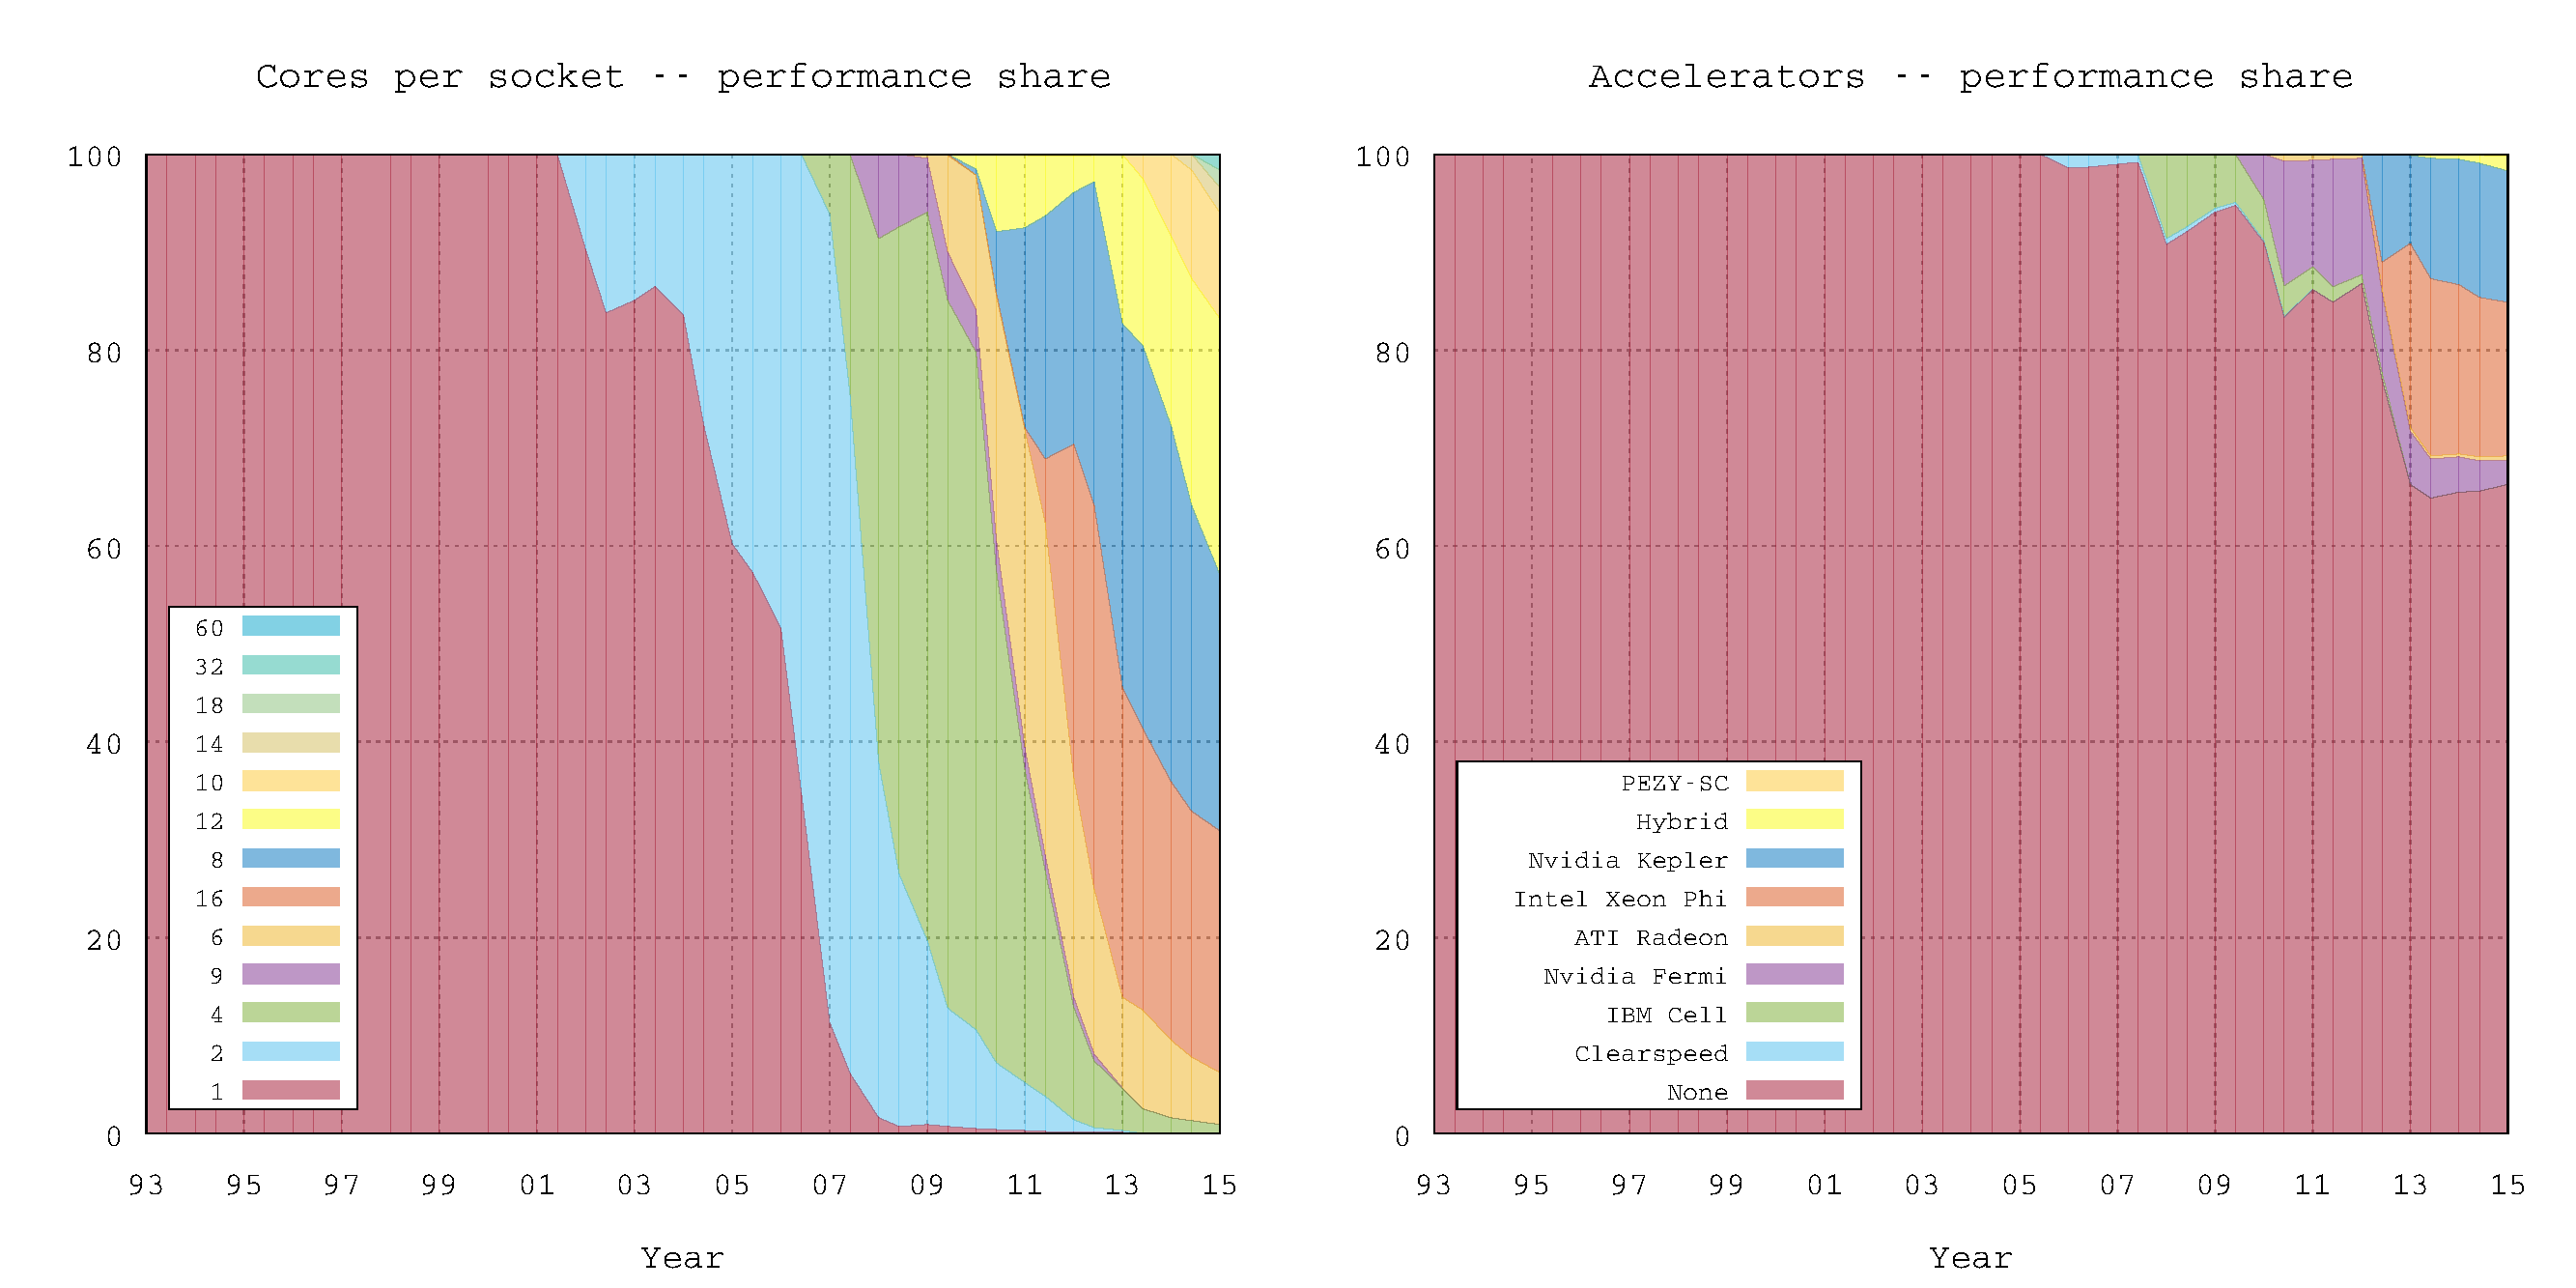
\includegraphics[width=0.9\textwidth]{top500}
%   \end{center}

%   According to the \dr{Top500 lists}, multicore
%   architectures introduced in 2001 nowadays represents 100 \% of
%   the performance share in the list. Accelerator, such as \db{GPU}
%   and \db{Xeon Phi devices}, started gaining interests in the HPC
%   community in 2005 and became very popular ever since.

% \end{frame}

\begin{frame}{Runtime systems}
  \begin{columns}
    \begin{column}{0.45\textwidth}
      \center
      \only<1>{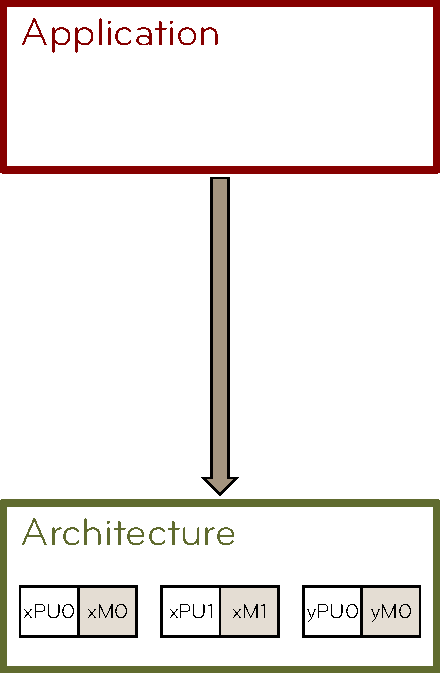
\includegraphics[width=\textwidth]{figures/rt_layers1}}%
      \only<2->{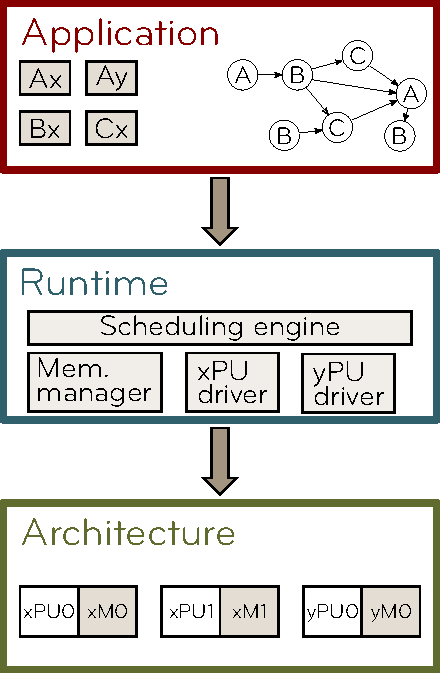
\includegraphics[width=\textwidth]{figures/rt_layers2}}%
    \end{column}
    \begin{column}{0.55\textwidth}
      \begin{itemize}
      \item<1->The classical approach is based on a mixture of
        technologies (e.g., MPI+OpenMP+CUDA) which.
        \begin{itemize}
        \item requires a big programming effort.
        \item is difficult to maintain and update.
        \item is prone to (performance) portability issues.
        \end{itemize}
      \item<2-> \dr{runtimes} provide an abstraction layer that hides
        the architecture details.
      \item<3-> the workload is expressed as a \dr{DAG} (Directed
        Acyclic Graph) of tasks.
        % where the dependencies are
        % \begin{itemize}
        % \item<3-> defined explicitly
        % \item<3-> defined through rules
        % \item<3-> automatically inferred
        % \end{itemize}
      \end{itemize}
    \end{column}
  \end{columns}
\end{frame}

\begin{frame}{Runtime systems and programming models}

  This approach has been assessed in the domain of \dr{dense
  linear algebra} and still represents a challenge for \dr{sparse
  algorithms}.

  \begin{itemize}
  \item \dr{Programming models}: \\ \db{Sequential Task Flow (STF)},
    Parametrized Tasks Graph (PTG) % recurssive, call-back
  \item \dr{Runtime systems}: \\ \db{StarPU}, PaRSEC, QUARK, KAAPI, StarSS,
    SuperGlue
  \item \dr{Research project}: \\ \db{SOLHAR (ANR-MN)}, NLAFET
    (H2020), INTERTWinE (H2020), SparseKafe (NSF)
  \item \dr{Scientific libraries}: \\ \texttt{qr\_mumps}, PasTiX,
    Chameleon, (D)PLASMA
  \end{itemize}

  \vspace{0.3cm}

  \uncover<2>{Recently added features of the OpenMP standard have been inspired by
  these efforts:
  \begin{itemize}
  \item OpenMP 3.0: the \texttt{task} construct
  \item OpenMP 4.0: the \texttt{depend} clause and
    \texttt{target} construct
  \item OpenMP 4.5: the \texttt{priority} clause
  \end{itemize}}

\end{frame}

\begin{frame}{Position of the thesis}

  \vspace{0.3cm}
  
  \begin{block}{Challenges}
    Achieve an efficient and portable implementation of a sparse,
    direct method, improve it by integrating new advanced features and
    achieve the porting on heterogeneous architectures.
  \end{block}

  \vspace{0.3cm}

  % \uncover<2->{Exploiting a pure \dr{STF} model on top of a modern \dr{runtime
    % system}:}
  \uncover<2->{Use a task-based parallel paradigm trough a
    \dr{runtime system}:}

  \vspace{0.1cm}

  \begin{itemize}
  % \item<2-> Improve the scalability of a sparse direct solver by
  %   introducing 2D, Communication Avoiding front factorization
  %   algorithms.
  \item<2-> Improve the scalability of a sparse direct solver by
    introducing 2D, Communication Avoiding algorithms.
  \item<3-> Devise algorithms for efficiently exploit the capabilities
    of \dr{heterogeneous systems}.
  \item<4-> Design and implement a reliable and efficient \alert{memory-aware}
    algorithm for controlling the memory consumption of the solver
    during a parallel execution.
  \item<5-> Develop tools for \alert{analyzing and evaluating} the performance and
    scaling of a parallel application on heterogeneous systems.
  \end{itemize}
  
\end{frame}

%%% Local Variables:
%%% mode: latex
%%% TeX-master: "defense"
%%% TeX-engine: xetex
%%% End:
